\chapter{Convolutional Neural Network}
\label{cha:conv}

Image recognition is a particularly challenging task. The naive approach would be to define set of features that an algorithm would recognize and then based on the results classify an object. For instance, if the task was to detect an handwritten digit, one could define set of shapes that a number can consist of. If the algorithm found double ``o'' shape it would mean that number ``8'' was recognized and so on. However, such approach fails due to the fact that there are countless variations of writing the same digit and what is more, each can be rotated or offset. It would require complex set of mappings for each and every scenario.

This is the point when \textbf{Convolutional Neural Networks (CNN)} come in handy. Their ability to learn complex, high-dimensional and non-linear mappings from huge collections of samples makes them perfect candidate for digit or any image recognition tasks. The typical CNN consists of one or more of \textbf{convolution} layer followed by \textbf{activation} and \textbf{pooling} layer. This is a part where \textbf{feature extraction} and \textbf{dimension reduction} is performed. Activation function ensures the nonlinearity of the output of convolution. The example of such network, capable of recognizing hand written digits, is \emph{LeNet-5} described by \emph{Yann Lecun et al.} \cite{GradientBasedLearningDigitRec} (figure \ref{fig:le-net-5}).

\begin{figure}[h]
    \centering
    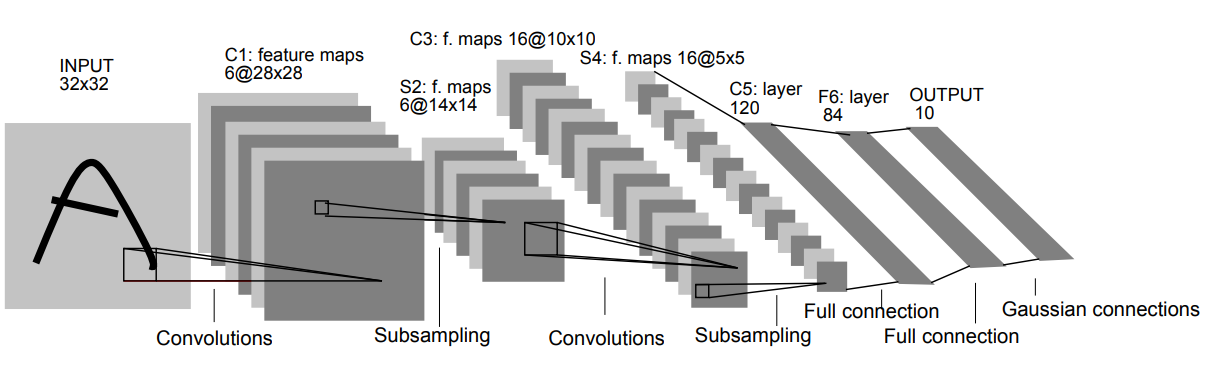
\includegraphics[width=14cm]{img/LeNet-5.png}
    \caption{LeNet-5, CNN for handwritten digits recognition. Source \cite{GradientBasedLearningDigitRec}}
    \label{fig:le-net-5}
\end{figure}

\section{Convolution}
\label{sec:convolution}

Convolution operation on a 3D tensor $H \times W \times D$ (2D image with R, G and B channels) applies a kernel, which is usually a $M \times N \times D$ matrix 
($0 \leq M \leq H, 0 \leq N \leq W$), on the top of spatial location $(0, 0, 0)$. Then products of corresponding elements overlapped by the kernel are computed in all $D$ channels and summed to get the result in this location. The next step is to move move the kernel top to bottom and left to right and perform the convolution operation in every spatial location.

Figure \ref{fig:conv-example} illustrates a convolution on an 2D $4 \times 3$ matrix with an $4 \times 2$ kernel and hopefully clarifies the whole concept. The process for the 3rd order tensor is analogical.

\begin{figure}[h]
    \centering
    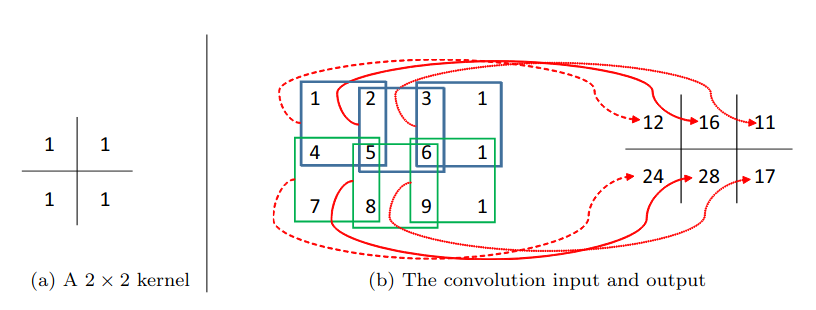
\includegraphics[width=14cm]{img/ConvExample.png}
    \caption{Convolution operation. Source \cite{Wu2017IntroductionTC}}
    \label{fig:conv-example}
\end{figure}

\subsection{The purpose of convolution}
\label{sub:purpose-of-convolution}

Applying convolutions with different kernels, also called feature extractors, enables do detect certain set of features from the image. The figure \ref{fig:conv-lenna} shows effect of applying a $3 \times 3 \times 3$ kernel (\ref{eq:conv-kernel})

\begin{equation}
    K = \begin{bmatrix}
            1 & 2 & 1 \\
            0 & 0 & 0 \\
            -1 & -2 & -1
        \end{bmatrix}
    \label{eq:conv-kernel}
\end{equation}

and a transposed $K^T$ on probably the most exploited woman on the internet, Lenna. This particular kernel detects and amplifies horizontal or vertical edges, but any type of kernel can be used. The next layer is usually a ReLU, which activates only for edges at a certain direction. Subsequent layers in network can activate for more complex group of features or even the entire objects like human face, cat or dog. 

Another advantage of convolution layer is that it is \textbf{spatially invariant}, which means that it is insensitive to feature position on a picture. If there were many objects at the same image, the feature would activate at multiple locations. What is more, the convolution network architecture encourages a parameter sharing. If the network learned to recognize an eye or a hand, it does not need to limit it to one particular type of eye (e.g. human eye). Instead the bottom layers may share patterns used to detect more abstract features in the next layers. In our example, the eye pattern can be used to detect a human, a cat or a dog.

All in all, convolution kernels combined with a deep and hierarchical structures are en extremely efficient tool for visual recognition tasks.

\begin{figure}[h]
    \centering
    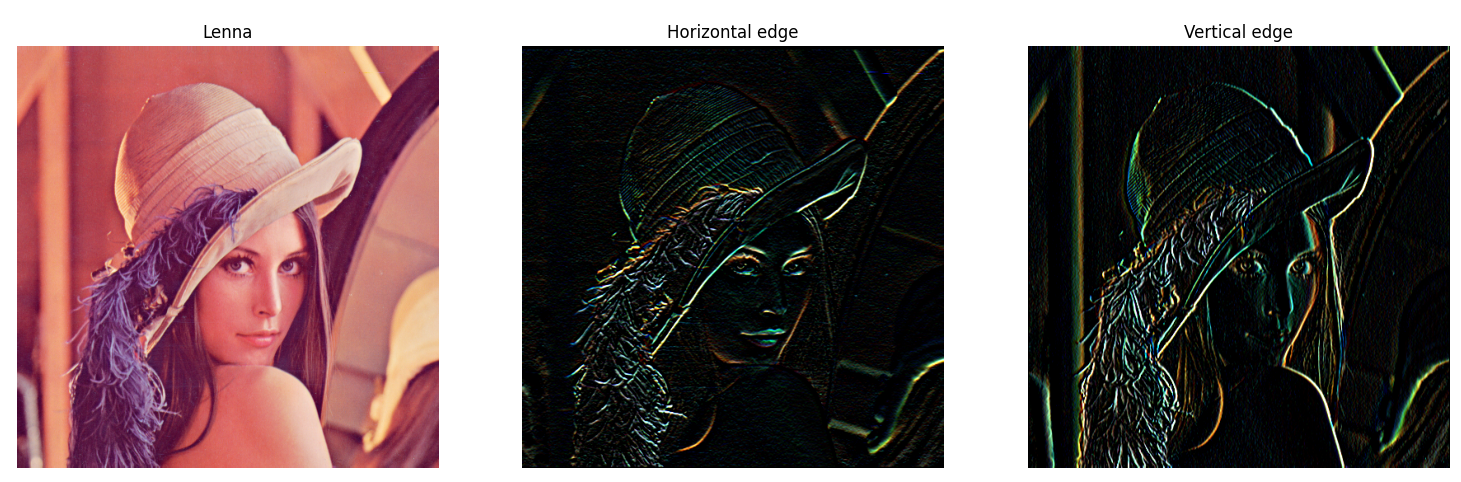
\includegraphics[width=16cm]{img/Lenna1.png}
    \caption{The Lenna image and the output of different convolution kernels}
    \label{fig:conv-lenna}
\end{figure}

\section{Activation}
\label{sec:conv-activation}

CNN adopted three main activation functions: \textbf{sigmoid}, \textbf{ReLU} and \textbf{PReLU}, shown at figure \ref{fig:conv-activation}. They have been described in a chapter \ref{sec:activation-function}, except the PReLU which is a parametric version of ReLU and is described in the appendix to this section.

\begin{figure}[h]
    \centering
    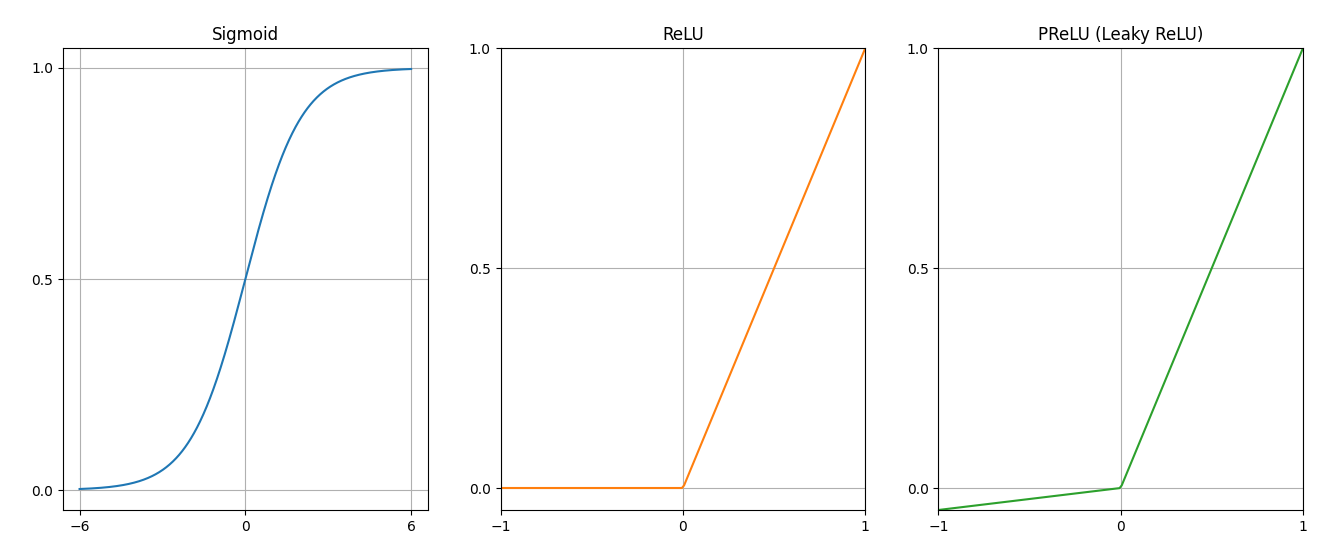
\includegraphics[width=16cm, height=6cm]{img/CNN-activations.png}
    \caption{Non-linear activations adopted by CNNs.}
    \label{fig:conv-activation}
\end{figure}

Every of them serve clip the output of convolution. Sigmoid squashes the output into the $[0, 1]$ interval. The ReLU sets the negative values to 0 and keeps the positive unchanged. The PReLU maps larger negative values to smaller ones by reducing the slope or the mapping function. It has been shown in the experiments that removing a non-linear operation significantly decreases the performance of CNN. Their importance have been described by \emph{C.-C. Jay Kuo} \cite{kuo2016understanding}, \emph{Kaiming He et al.} \cite{he2015delving} and many others.


\subsubsection*{PReLU}
\label{sub2:prelu}

The \textbf{Parametric Rectifier Linear Unit} function has been introduced in ``\emph{Delving Deep into Rectifiers: Surpassing Human-Level Performance on ImageNet Classification}'' \cite{he2015delving}. The authors of the publication state that using this particular activation they managed to outperform human at image recognition of \emph{ImageNet} \footnote{1000-class ImageNet 2012 dataset} dataset.

The function is defined as

\begin{equation}
    f(y_i) = 
        \begin{cases}
        y_i & y_i > 0 \\
        a_i y_i & y_i \leq 0
        \end{cases}
\end{equation}

where:

$y_i$ is the activation input on the \emph{i-th} channel,

$a_i$ is the coefficient controlling the slope of the negative part. 

\section{Pooling}
\label{sec:conv-pooling}

This layer is mainly responsible for a shift invariance and spatial dimension reduction. In other words, a processed image has a reduced size containing only detected features by the previous layers. This reduces the calculations complexity and enables the network to focus only on important parts of an image, dropping the remaining part. If the task was to find a Wally, there is no need to keep track of information about the location where he stands.

Originally, pooling was performed by \textbf{subsampling} layers. Neurons receive an input from a small non-overlapping receptive field of a previous layer. Then each neuron computes a sum of its inputs, multiplies it by a trainable coefficient, adds a trainable bias and passes the result through non-linear transfer function. Such approach was implemented in \emph{LeNet-5} \cite{GradientBasedLearningDigitRec}.

\begin{equation}
    a_j = tanh\left(\beta \sum_{N \times N} a_i^{N \times N} + b \right)
\end{equation}

Recently, subsampling layer has been replaced by \textbf{max pooling} operation. It is much simpler in foundations since it only propagates the maximum of the receptive field to the next layer. Despite that, as \emph{Dominik Scherer et al.} \cite{MaxPool} showed, it is superior for capturing invariances in image data to a subsampling operations

\begin{equation}
    a_j = \max_{N \times N} \left( a_i^{N \times N} u(n, n) \right)
\end{equation}

where $u(x, y)$ is a transfer window function. In both cases the output is a lower resolution image.
